% Options for packages loaded elsewhere
\PassOptionsToPackage{unicode}{hyperref}
\PassOptionsToPackage{hyphens}{url}
%
\documentclass[
]{article}
\usepackage{amsmath,amssymb}
\usepackage{lmodern}
\usepackage{iftex}
\ifPDFTeX
  \usepackage[T1]{fontenc}
  \usepackage[utf8]{inputenc}
  \usepackage{textcomp} % provide euro and other symbols
\else % if luatex or xetex
  \usepackage{unicode-math}
  \defaultfontfeatures{Scale=MatchLowercase}
  \defaultfontfeatures[\rmfamily]{Ligatures=TeX,Scale=1}
\fi
% Use upquote if available, for straight quotes in verbatim environments
\IfFileExists{upquote.sty}{\usepackage{upquote}}{}
\IfFileExists{microtype.sty}{% use microtype if available
  \usepackage[]{microtype}
  \UseMicrotypeSet[protrusion]{basicmath} % disable protrusion for tt fonts
}{}
\makeatletter
\@ifundefined{KOMAClassName}{% if non-KOMA class
  \IfFileExists{parskip.sty}{%
    \usepackage{parskip}
  }{% else
    \setlength{\parindent}{0pt}
    \setlength{\parskip}{6pt plus 2pt minus 1pt}}
}{% if KOMA class
  \KOMAoptions{parskip=half}}
\makeatother
\usepackage{xcolor}
\usepackage[margin=1in]{geometry}
\usepackage{color}
\usepackage{fancyvrb}
\newcommand{\VerbBar}{|}
\newcommand{\VERB}{\Verb[commandchars=\\\{\}]}
\DefineVerbatimEnvironment{Highlighting}{Verbatim}{commandchars=\\\{\}}
% Add ',fontsize=\small' for more characters per line
\usepackage{framed}
\definecolor{shadecolor}{RGB}{248,248,248}
\newenvironment{Shaded}{\begin{snugshade}}{\end{snugshade}}
\newcommand{\AlertTok}[1]{\textcolor[rgb]{0.94,0.16,0.16}{#1}}
\newcommand{\AnnotationTok}[1]{\textcolor[rgb]{0.56,0.35,0.01}{\textbf{\textit{#1}}}}
\newcommand{\AttributeTok}[1]{\textcolor[rgb]{0.77,0.63,0.00}{#1}}
\newcommand{\BaseNTok}[1]{\textcolor[rgb]{0.00,0.00,0.81}{#1}}
\newcommand{\BuiltInTok}[1]{#1}
\newcommand{\CharTok}[1]{\textcolor[rgb]{0.31,0.60,0.02}{#1}}
\newcommand{\CommentTok}[1]{\textcolor[rgb]{0.56,0.35,0.01}{\textit{#1}}}
\newcommand{\CommentVarTok}[1]{\textcolor[rgb]{0.56,0.35,0.01}{\textbf{\textit{#1}}}}
\newcommand{\ConstantTok}[1]{\textcolor[rgb]{0.00,0.00,0.00}{#1}}
\newcommand{\ControlFlowTok}[1]{\textcolor[rgb]{0.13,0.29,0.53}{\textbf{#1}}}
\newcommand{\DataTypeTok}[1]{\textcolor[rgb]{0.13,0.29,0.53}{#1}}
\newcommand{\DecValTok}[1]{\textcolor[rgb]{0.00,0.00,0.81}{#1}}
\newcommand{\DocumentationTok}[1]{\textcolor[rgb]{0.56,0.35,0.01}{\textbf{\textit{#1}}}}
\newcommand{\ErrorTok}[1]{\textcolor[rgb]{0.64,0.00,0.00}{\textbf{#1}}}
\newcommand{\ExtensionTok}[1]{#1}
\newcommand{\FloatTok}[1]{\textcolor[rgb]{0.00,0.00,0.81}{#1}}
\newcommand{\FunctionTok}[1]{\textcolor[rgb]{0.00,0.00,0.00}{#1}}
\newcommand{\ImportTok}[1]{#1}
\newcommand{\InformationTok}[1]{\textcolor[rgb]{0.56,0.35,0.01}{\textbf{\textit{#1}}}}
\newcommand{\KeywordTok}[1]{\textcolor[rgb]{0.13,0.29,0.53}{\textbf{#1}}}
\newcommand{\NormalTok}[1]{#1}
\newcommand{\OperatorTok}[1]{\textcolor[rgb]{0.81,0.36,0.00}{\textbf{#1}}}
\newcommand{\OtherTok}[1]{\textcolor[rgb]{0.56,0.35,0.01}{#1}}
\newcommand{\PreprocessorTok}[1]{\textcolor[rgb]{0.56,0.35,0.01}{\textit{#1}}}
\newcommand{\RegionMarkerTok}[1]{#1}
\newcommand{\SpecialCharTok}[1]{\textcolor[rgb]{0.00,0.00,0.00}{#1}}
\newcommand{\SpecialStringTok}[1]{\textcolor[rgb]{0.31,0.60,0.02}{#1}}
\newcommand{\StringTok}[1]{\textcolor[rgb]{0.31,0.60,0.02}{#1}}
\newcommand{\VariableTok}[1]{\textcolor[rgb]{0.00,0.00,0.00}{#1}}
\newcommand{\VerbatimStringTok}[1]{\textcolor[rgb]{0.31,0.60,0.02}{#1}}
\newcommand{\WarningTok}[1]{\textcolor[rgb]{0.56,0.35,0.01}{\textbf{\textit{#1}}}}
\usepackage{graphicx}
\makeatletter
\def\maxwidth{\ifdim\Gin@nat@width>\linewidth\linewidth\else\Gin@nat@width\fi}
\def\maxheight{\ifdim\Gin@nat@height>\textheight\textheight\else\Gin@nat@height\fi}
\makeatother
% Scale images if necessary, so that they will not overflow the page
% margins by default, and it is still possible to overwrite the defaults
% using explicit options in \includegraphics[width, height, ...]{}
\setkeys{Gin}{width=\maxwidth,height=\maxheight,keepaspectratio}
% Set default figure placement to htbp
\makeatletter
\def\fps@figure{htbp}
\makeatother
\setlength{\emergencystretch}{3em} % prevent overfull lines
\providecommand{\tightlist}{%
  \setlength{\itemsep}{0pt}\setlength{\parskip}{0pt}}
\setcounter{secnumdepth}{-\maxdimen} % remove section numbering
\ifLuaTeX
  \usepackage{selnolig}  % disable illegal ligatures
\fi
\IfFileExists{bookmark.sty}{\usepackage{bookmark}}{\usepackage{hyperref}}
\IfFileExists{xurl.sty}{\usepackage{xurl}}{} % add URL line breaks if available
\urlstyle{same} % disable monospaced font for URLs
\hypersetup{
  pdftitle={Time-Series Modelling},
  pdfauthor={Ralf Becker},
  hidelinks,
  pdfcreator={LaTeX via pandoc}}

\title{Time-Series Modelling}
\author{Ralf Becker}
\date{April 2023}

\begin{document}
\maketitle

\begin{Shaded}
\begin{Highlighting}[]
\FunctionTok{library}\NormalTok{(tidyverse)}
\end{Highlighting}
\end{Shaded}

\begin{verbatim}
## Warning: package 'tidyverse' was built under R version 4.2.3
\end{verbatim}

\begin{verbatim}
## Warning: package 'ggplot2' was built under R version 4.2.3
\end{verbatim}

\begin{verbatim}
## Warning: package 'tibble' was built under R version 4.2.3
\end{verbatim}

\begin{verbatim}
## Warning: package 'readr' was built under R version 4.2.3
\end{verbatim}

\begin{verbatim}
## Warning: package 'dplyr' was built under R version 4.2.3
\end{verbatim}

\begin{verbatim}
## Warning: package 'lubridate' was built under R version 4.2.3
\end{verbatim}

\begin{verbatim}
## -- Attaching core tidyverse packages ------------------------ tidyverse 2.0.0 --
## v dplyr     1.1.1     v readr     2.1.4
## v forcats   1.0.0     v stringr   1.5.0
## v ggplot2   3.4.2     v tibble    3.2.1
## v lubridate 1.9.2     v tidyr     1.3.0
## v purrr     1.0.1     
## -- Conflicts ------------------------------------------ tidyverse_conflicts() --
## x dplyr::filter() masks stats::filter()
## x dplyr::lag()    masks stats::lag()
## i Use the ]8;;http://conflicted.r-lib.org/conflicted package]8;; to force all conflicts to become errors
\end{verbatim}

\begin{Shaded}
\begin{Highlighting}[]
\FunctionTok{library}\NormalTok{(ggplot2)}
\FunctionTok{library}\NormalTok{(pdfetch)}
\end{Highlighting}
\end{Shaded}

\begin{verbatim}
## Warning: package 'pdfetch' was built under R version 4.2.3
\end{verbatim}

\begin{Shaded}
\begin{Highlighting}[]
\FunctionTok{library}\NormalTok{(xts)}
\end{Highlighting}
\end{Shaded}

\begin{verbatim}
## Warning: package 'xts' was built under R version 4.2.3
\end{verbatim}

\begin{verbatim}
## Loading required package: zoo
\end{verbatim}

\begin{verbatim}
## Warning: package 'zoo' was built under R version 4.2.3
\end{verbatim}

\begin{verbatim}
## 
## Attaching package: 'zoo'
## 
## The following objects are masked from 'package:base':
## 
##     as.Date, as.Date.numeric
## 
## 
## ################################### WARNING ###################################
## # We noticed you have dplyr installed. The dplyr lag() function breaks how    #
## # base R's lag() function is supposed to work, which breaks lag(my_xts).      #
## #                                                                             #
## # Calls to lag(my_xts) that you enter or source() into this session won't     #
## # work correctly.                                                             #
## #                                                                             #
## # All package code is unaffected because it is protected by the R namespace   #
## # mechanism.                                                                  #
## #                                                                             #
## # Set `options(xts.warn_dplyr_breaks_lag = FALSE)` to suppress this warning.  #
## #                                                                             #
## # You can use stats::lag() to make sure you're not using dplyr::lag(), or you #
## # can add conflictRules('dplyr', exclude = 'lag') to your .Rprofile to stop   #
## # dplyr from breaking base R's lag() function.                                #
## ################################### WARNING ###################################
## 
## Attaching package: 'xts'
## 
## The following objects are masked from 'package:dplyr':
## 
##     first, last
\end{verbatim}

\begin{Shaded}
\begin{Highlighting}[]
\FunctionTok{library}\NormalTok{(AER)          }\CommentTok{\# access to HS robust standard errors}
\end{Highlighting}
\end{Shaded}

\begin{verbatim}
## Loading required package: car
\end{verbatim}

\begin{verbatim}
## Warning: package 'car' was built under R version 4.2.3
\end{verbatim}

\begin{verbatim}
## Loading required package: carData
## 
## Attaching package: 'car'
## 
## The following object is masked from 'package:dplyr':
## 
##     recode
## 
## The following object is masked from 'package:purrr':
## 
##     some
## 
## Loading required package: lmtest
## Loading required package: sandwich
## Loading required package: survival
\end{verbatim}

\begin{Shaded}
\begin{Highlighting}[]
\FunctionTok{library}\NormalTok{(stargazer)}
\end{Highlighting}
\end{Shaded}

\begin{verbatim}
## 
## Please cite as: 
## 
##  Hlavac, Marek (2022). stargazer: Well-Formatted Regression and Summary Statistics Tables.
##  R package version 5.2.3. https://CRAN.R-project.org/package=stargazer
\end{verbatim}

\begin{Shaded}
\begin{Highlighting}[]
\FunctionTok{source}\NormalTok{(}\StringTok{"stargazer\_HC.r"}\NormalTok{)  }\CommentTok{\# includes the robust regression display}
\FunctionTok{source}\NormalTok{(}\StringTok{"stargazer\_HAC.r"}\NormalTok{)  }\CommentTok{\# includes the Newey{-}West standard errors}
\FunctionTok{library}\NormalTok{(gridExtra)  }\CommentTok{\# required for the combination of ggplots}
\end{Highlighting}
\end{Shaded}

\begin{verbatim}
## 
## Attaching package: 'gridExtra'
## 
## The following object is masked from 'package:dplyr':
## 
##     combine
\end{verbatim}

\hypertarget{import-data-and-look-at-acf}{%
\section{Import data and look at
ACF}\label{import-data-and-look-at-acf}}

When you get data from the ONS you need to know what the series id is
and in which ONS dataset you can find these data. The way to find out
what that info is it is best to go to (the ONS time series
tool){[}\url{https://www.ons.gov.uk/timeseriestool}{]}.

For instance we can get real GDP data (id: AMBI) from the UKEA databank.

\begin{Shaded}
\begin{Highlighting}[]
\NormalTok{rGDP }\OtherTok{\textless{}{-}} \FunctionTok{pdfetch\_ONS}\NormalTok{(}\StringTok{"ABMI"}\NormalTok{,}\StringTok{"UKEA"}\NormalTok{)  }
\FunctionTok{periodicity}\NormalTok{(rGDP)   }\CommentTok{\# check data availability}
\end{Highlighting}
\end{Shaded}

\begin{verbatim}
## Quarterly periodicity from 1955-03-31 to 2022-12-31
\end{verbatim}

\begin{Shaded}
\begin{Highlighting}[]
\FunctionTok{names}\NormalTok{(rGDP) }\OtherTok{\textless{}{-}} \StringTok{"real GDP"} \CommentTok{\# give a sensible name}

\CommentTok{\# keep all the data including 2020{-}Q3}
\CommentTok{\# this was the last observation available at the time this was written}
\CommentTok{\# remove this line if you want to use updated data}
\NormalTok{rGDP }\OtherTok{\textless{}{-}}\NormalTok{ rGDP[}\StringTok{"/2022{-}12"}\NormalTok{]  }

\CommentTok{\# we prepare the data for being kept in long format}
\CommentTok{\# that is useful for plotting in ggplot}
\NormalTok{rGDP\_l }\OtherTok{\textless{}{-}} \FunctionTok{data.frame}\NormalTok{(}\FunctionTok{index}\NormalTok{(rGDP),}\FunctionTok{stack}\NormalTok{(}\FunctionTok{as.data.frame}\NormalTok{(}\FunctionTok{coredata}\NormalTok{(rGDP))))}
\CommentTok{\# Give sensible names to columns}
\FunctionTok{names}\NormalTok{(rGDP\_l)[}\DecValTok{1}\NormalTok{] }\OtherTok{\textless{}{-}} \StringTok{"Date"}   \CommentTok{\# first col will have date}
\FunctionTok{names}\NormalTok{(rGDP\_l)[}\DecValTok{2}\NormalTok{] }\OtherTok{\textless{}{-}} \StringTok{"Value"}  \CommentTok{\# second col will have value}
\FunctionTok{names}\NormalTok{(rGDP\_l)[}\DecValTok{3}\NormalTok{] }\OtherTok{\textless{}{-}} \StringTok{"id"}     \CommentTok{\# third col will have series name}
\end{Highlighting}
\end{Shaded}

Let's look at the series

\begin{Shaded}
\begin{Highlighting}[]
\FunctionTok{ggplot}\NormalTok{(rGDP\_l,}\FunctionTok{aes}\NormalTok{(}\AttributeTok{x =}\NormalTok{Date, }\AttributeTok{y=}\NormalTok{Value)) }\SpecialCharTok{+} 
  \FunctionTok{geom\_line}\NormalTok{(}\AttributeTok{colour =} \StringTok{"blue"}\NormalTok{,}\AttributeTok{size =} \FloatTok{1.5}\NormalTok{) }\SpecialCharTok{+}
  \FunctionTok{ggtitle}\NormalTok{(}\StringTok{"UK real GDP"}\NormalTok{) }\SpecialCharTok{+}
  \FunctionTok{theme\_bw}\NormalTok{()}
\end{Highlighting}
\end{Shaded}

\begin{verbatim}
## Warning: Using `size` aesthetic for lines was deprecated in ggplot2 3.4.0.
## i Please use `linewidth` instead.
## This warning is displayed once every 8 hours.
## Call `lifecycle::last_lifecycle_warnings()` to see where this warning was
## generated.
\end{verbatim}

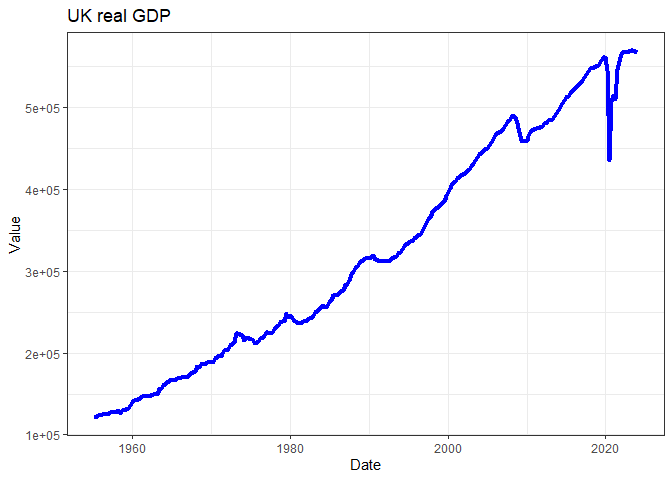
\includegraphics{TS_Modelling_files/figure-latex/unnamed-chunk-3-1.pdf}

If you want to plot a subsample of the data only, the easiest way to do
that is to use the \texttt{subset} function as you call the data into
the \texttt{ggplot} function. Compare what has changed in the code and
figure out what the \texttt{subset} function did.

\begin{Shaded}
\begin{Highlighting}[]
\FunctionTok{ggplot}\NormalTok{(}\FunctionTok{subset}\NormalTok{(rGDP\_l, Date }\SpecialCharTok{\textgreater{}}\StringTok{"2000{-}01{-}01"}\NormalTok{),}\FunctionTok{aes}\NormalTok{(}\AttributeTok{x =}\NormalTok{Date, }\AttributeTok{y=}\NormalTok{Value)) }\SpecialCharTok{+} 
  \FunctionTok{geom\_line}\NormalTok{(}\AttributeTok{colour =} \StringTok{"blue"}\NormalTok{,}\AttributeTok{size =} \FloatTok{1.5}\NormalTok{) }\SpecialCharTok{+}
  \FunctionTok{ggtitle}\NormalTok{(}\StringTok{"UK real GDP"}\NormalTok{) }\SpecialCharTok{+}
  \FunctionTok{theme\_bw}\NormalTok{()}
\end{Highlighting}
\end{Shaded}

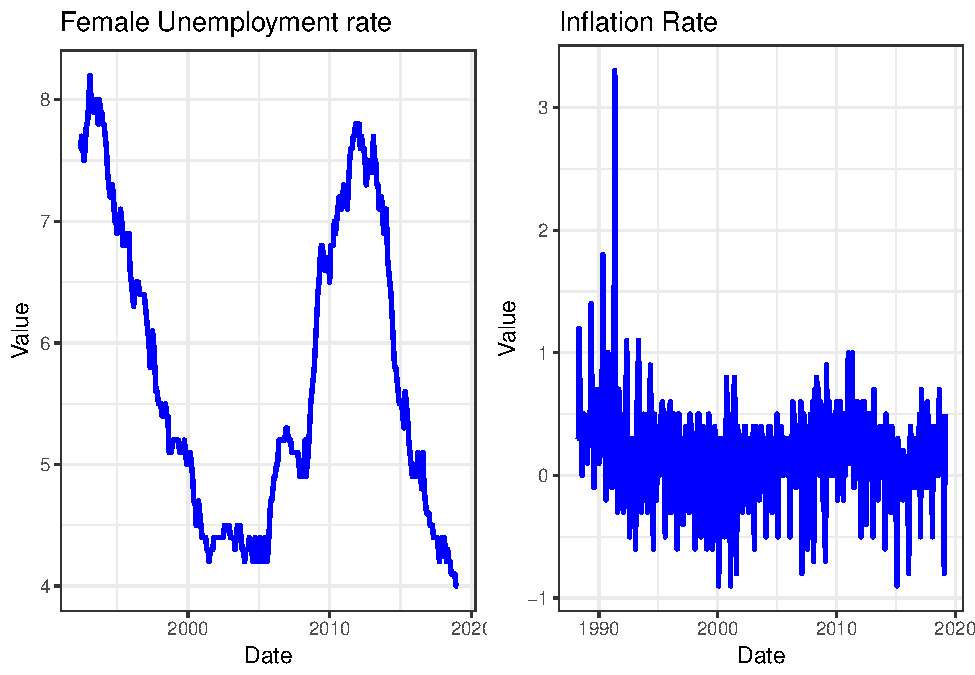
\includegraphics{TS_Modelling_files/figure-latex/unnamed-chunk-4-1.pdf}

Can you change the above code such that only the GDP from 2005 onwards
is shown?

Let's calculate the autocorrelation function:

\begin{Shaded}
\begin{Highlighting}[]
\NormalTok{temp\_acf }\OtherTok{\textless{}{-}} \FunctionTok{acf}\NormalTok{(rGDP)}
\end{Highlighting}
\end{Shaded}

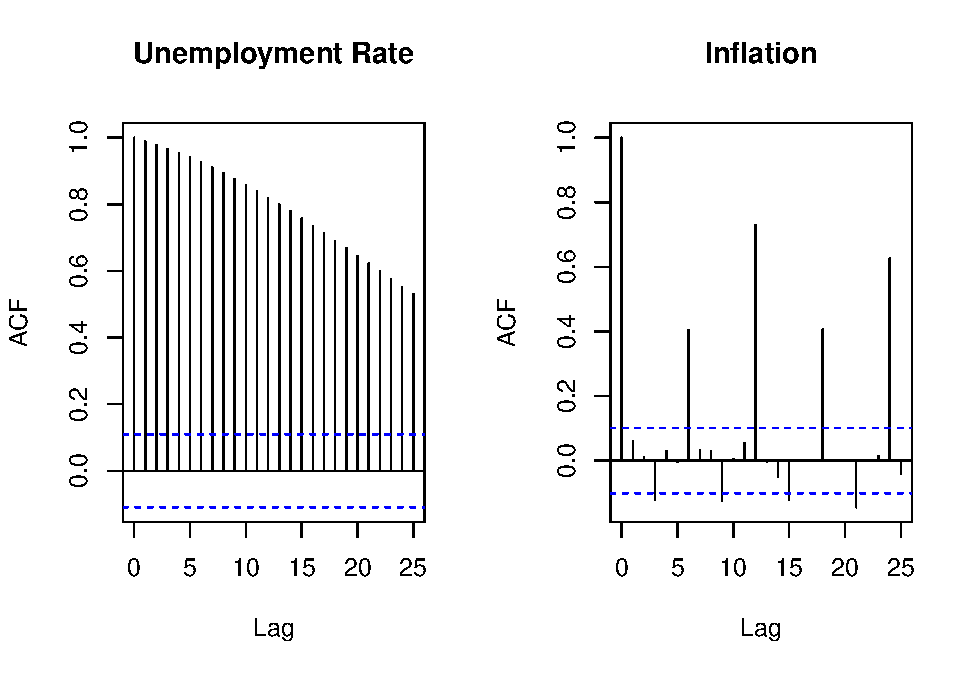
\includegraphics{TS_Modelling_files/figure-latex/unnamed-chunk-5-1.pdf}

Now we download female unemployment rates and monthly inflation rates
from the ONS database. On both occasions we put the

\begin{Shaded}
\begin{Highlighting}[]
\CommentTok{\# Download: Female unemployment rate (YCPL in database LMS)}
\NormalTok{ur\_female }\OtherTok{\textless{}{-}} \FunctionTok{pdfetch\_ONS}\NormalTok{(}\StringTok{"YCPL"}\NormalTok{,}\StringTok{"LMS"}\NormalTok{)}
\FunctionTok{names}\NormalTok{(ur\_female) }\OtherTok{\textless{}{-}} \StringTok{"Unemp Rate (female)"}
\FunctionTok{periodicity}\NormalTok{(ur\_female)}
\end{Highlighting}
\end{Shaded}

\begin{verbatim}
## Monthly periodicity from 1992-04-30 to 2023-01-31
\end{verbatim}

\begin{Shaded}
\begin{Highlighting}[]
\CommentTok{\# keep all the data including 2022{-}Jan}
\CommentTok{\# this was the last observation available at the time this was written}
\CommentTok{\# remove this line if you want to use updated data}
\NormalTok{ur\_female }\OtherTok{\textless{}{-}}\NormalTok{ ur\_female[}\StringTok{"/2022{-}12"}\NormalTok{]  }

\NormalTok{ur\_female\_l }\OtherTok{\textless{}{-}} \FunctionTok{data.frame}\NormalTok{(}\FunctionTok{index}\NormalTok{(ur\_female),}\FunctionTok{stack}\NormalTok{(}\FunctionTok{as.data.frame}\NormalTok{(}\FunctionTok{coredata}\NormalTok{(ur\_female))))}
\FunctionTok{names}\NormalTok{(ur\_female\_l)[}\DecValTok{1}\NormalTok{] }\OtherTok{\textless{}{-}} \StringTok{"Date"}
\FunctionTok{names}\NormalTok{(ur\_female\_l)[}\DecValTok{2}\NormalTok{] }\OtherTok{\textless{}{-}} \StringTok{"Value"}
\FunctionTok{names}\NormalTok{(ur\_female\_l)[}\DecValTok{3}\NormalTok{] }\OtherTok{\textless{}{-}} \StringTok{"id"}

\CommentTok{\# Download: Inflation rate (D7OE in database MM23)}
\NormalTok{infl }\OtherTok{\textless{}{-}} \FunctionTok{pdfetch\_ONS}\NormalTok{(}\StringTok{"D7OE"}\NormalTok{,}\StringTok{"MM23"}\NormalTok{)}
\FunctionTok{names}\NormalTok{(infl) }\OtherTok{\textless{}{-}} \StringTok{"CPI Inflation"}
\FunctionTok{periodicity}\NormalTok{(infl)}
\end{Highlighting}
\end{Shaded}

\begin{verbatim}
## Monthly periodicity from 1988-02-29 to 2023-02-28
\end{verbatim}

\begin{Shaded}
\begin{Highlighting}[]
\CommentTok{\# keep all the data including 2022{-}jan}
\CommentTok{\# this was the last observation available at the time this was written}
\CommentTok{\# remove this line if you want to use updated data}
\NormalTok{infl }\OtherTok{\textless{}{-}}\NormalTok{ infl[}\StringTok{"/2022{-}12"}\NormalTok{]  }

\NormalTok{infl\_l }\OtherTok{\textless{}{-}} \FunctionTok{data.frame}\NormalTok{(}\FunctionTok{index}\NormalTok{(infl),}\FunctionTok{stack}\NormalTok{(}\FunctionTok{as.data.frame}\NormalTok{(}\FunctionTok{coredata}\NormalTok{(infl))))}
\FunctionTok{names}\NormalTok{(infl\_l)[}\DecValTok{1}\NormalTok{] }\OtherTok{\textless{}{-}} \StringTok{"Date"}
\FunctionTok{names}\NormalTok{(infl\_l)[}\DecValTok{2}\NormalTok{] }\OtherTok{\textless{}{-}} \StringTok{"Value"}
\FunctionTok{names}\NormalTok{(infl\_l)[}\DecValTok{3}\NormalTok{] }\OtherTok{\textless{}{-}} \StringTok{"id"}
\end{Highlighting}
\end{Shaded}

Now we put both series into one dataframe by attaching the individual
dataframes. We can do this as we gave identical names to the three
columns in both dataframes.

\begin{Shaded}
\begin{Highlighting}[]
\NormalTok{data\_l }\OtherTok{\textless{}{-}} \FunctionTok{rbind}\NormalTok{(rGDP\_l,ur\_female\_l)}
\NormalTok{data\_l }\OtherTok{\textless{}{-}} \FunctionTok{rbind}\NormalTok{(data\_l,infl\_l)}
\end{Highlighting}
\end{Shaded}

Now we produce some time series plots and ACF functions

\begin{Shaded}
\begin{Highlighting}[]
\NormalTok{p1 }\OtherTok{\textless{}{-}} \FunctionTok{ggplot}\NormalTok{(data\_l[data\_l}\SpecialCharTok{$}\NormalTok{id }\SpecialCharTok{==} \StringTok{"Unemp Rate (female)"}\NormalTok{,],}\FunctionTok{aes}\NormalTok{(}\AttributeTok{x =}\NormalTok{Date, }\AttributeTok{y=}\NormalTok{Value)) }\SpecialCharTok{+} 
  \FunctionTok{geom\_line}\NormalTok{(}\AttributeTok{colour =} \StringTok{"blue"}\NormalTok{,}\AttributeTok{size =} \FloatTok{1.0}\NormalTok{) }\SpecialCharTok{+}
  \FunctionTok{ggtitle}\NormalTok{(}\StringTok{"Female Unemployment rate"}\NormalTok{) }\SpecialCharTok{+}
  \FunctionTok{theme\_bw}\NormalTok{()}

\NormalTok{p2 }\OtherTok{\textless{}{-}} \FunctionTok{ggplot}\NormalTok{(data\_l[data\_l}\SpecialCharTok{$}\NormalTok{id }\SpecialCharTok{==} \StringTok{"CPI Inflation"}\NormalTok{,],}\FunctionTok{aes}\NormalTok{(}\AttributeTok{x =}\NormalTok{Date, }\AttributeTok{y=}\NormalTok{Value)) }\SpecialCharTok{+} 
  \FunctionTok{geom\_line}\NormalTok{(}\AttributeTok{colour =} \StringTok{"blue"}\NormalTok{,}\AttributeTok{size =} \FloatTok{1.0}\NormalTok{) }\SpecialCharTok{+}
  \FunctionTok{ggtitle}\NormalTok{(}\StringTok{"Inflation Rate"}\NormalTok{) }\SpecialCharTok{+}
  \FunctionTok{theme\_bw}\NormalTok{()}

\FunctionTok{grid.arrange}\NormalTok{(p1, p2, }\AttributeTok{nrow=}\DecValTok{1}\NormalTok{, }\AttributeTok{ncol=}\DecValTok{2}\NormalTok{)}
\end{Highlighting}
\end{Shaded}

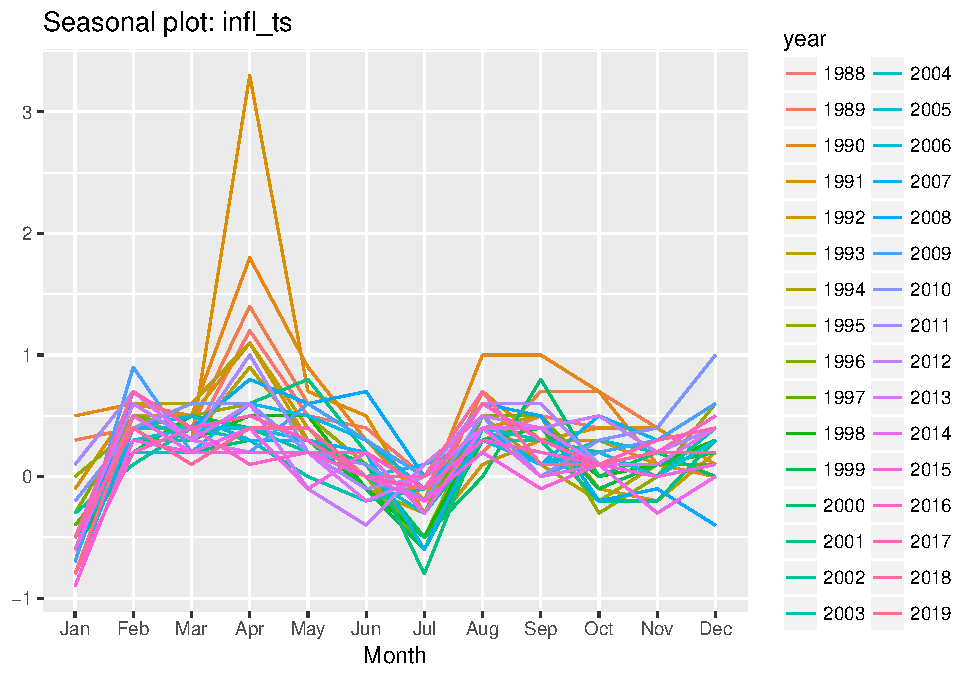
\includegraphics{TS_Modelling_files/figure-latex/unnamed-chunk-8-1.pdf}
The \texttt{grid.arrange(p1,\ p2,\ nrow=1,\ ncol=2)} line in the code
helped us to set the two images next to each other. That is very nice
and often useful when you present data. This sort of effect can be
achieved in different ways. It is important to realise that usually you
can do the same think in R in different ways. So let us present such a
different way. Below it is the \texttt{par(mfrow=c(1,2))} line which
tells R that the next plots should be presented in a 1 by 2 frame.

\begin{Shaded}
\begin{Highlighting}[]
\FunctionTok{par}\NormalTok{(}\AttributeTok{mfrow=}\FunctionTok{c}\NormalTok{(}\DecValTok{1}\NormalTok{,}\DecValTok{2}\NormalTok{))}

\FunctionTok{acf}\NormalTok{(ur\_female,}\AttributeTok{main =} \StringTok{"Unemployment Rate"}\NormalTok{)}
\FunctionTok{acf}\NormalTok{(infl, }\AttributeTok{main =} \StringTok{"Inflation"}\NormalTok{)}
\end{Highlighting}
\end{Shaded}

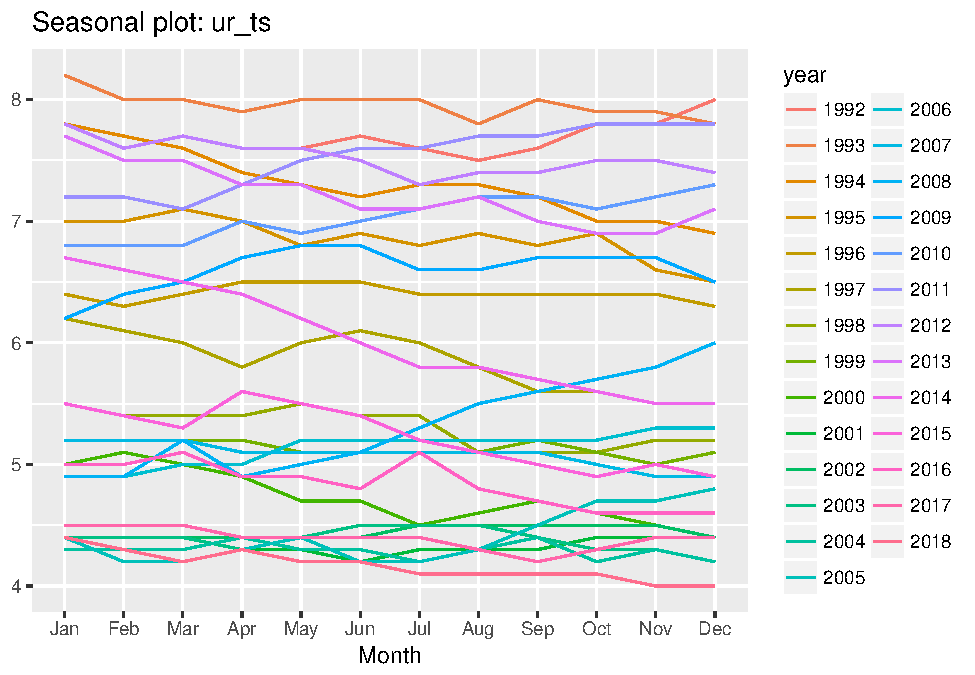
\includegraphics{TS_Modelling_files/figure-latex/unnamed-chunk-9-1.pdf}

It will be interesting to see what happens when we difference data
series (or often their logs).

\begin{Shaded}
\begin{Highlighting}[]
\NormalTok{g\_rGDP }\OtherTok{\textless{}{-}}\FunctionTok{diff}\NormalTok{(}\FunctionTok{log}\NormalTok{(rGDP))}
\FunctionTok{names}\NormalTok{(g\_rGDP) }\OtherTok{\textless{}{-}} \StringTok{"GDP, quarterly growth rate"}
\NormalTok{g\_ur\_female }\OtherTok{\textless{}{-}}\FunctionTok{diff}\NormalTok{(}\FunctionTok{log}\NormalTok{(ur\_female))}
\FunctionTok{names}\NormalTok{(g\_ur\_female) }\OtherTok{\textless{}{-}} \StringTok{"Growth in Unemp Rate (female)"}
\end{Highlighting}
\end{Shaded}

\begin{Shaded}
\begin{Highlighting}[]
\FunctionTok{par}\NormalTok{(}\AttributeTok{mfrow=}\FunctionTok{c}\NormalTok{(}\DecValTok{1}\NormalTok{,}\DecValTok{2}\NormalTok{))}

\FunctionTok{acf}\NormalTok{(g\_rGDP,}\AttributeTok{main =} \StringTok{"GDP, growth"}\NormalTok{)}
\FunctionTok{acf}\NormalTok{(g\_ur\_female, }\AttributeTok{main =} \StringTok{"Unemployment Rate, growth"}\NormalTok{)}
\end{Highlighting}
\end{Shaded}

When you do this you will get an error message as the differencing
created a missing value in the \texttt{g\_rGDP} and
\texttt{g\_ur\_female} series and the \texttt{acf} function really
dislikes missing values. Hence we need to tell it to ignore these.

\begin{Shaded}
\begin{Highlighting}[]
\FunctionTok{par}\NormalTok{(}\AttributeTok{mfrow=}\FunctionTok{c}\NormalTok{(}\DecValTok{2}\NormalTok{,}\DecValTok{2}\NormalTok{))}
\FunctionTok{plot}\NormalTok{(g\_rGDP)}
\FunctionTok{plot}\NormalTok{(g\_ur\_female)}
\FunctionTok{acf}\NormalTok{(g\_rGDP,}\AttributeTok{main =} \StringTok{"GDP, growth"}\NormalTok{, }\AttributeTok{na.action =}\NormalTok{ na.pass)}
\FunctionTok{acf}\NormalTok{(g\_ur\_female, }\AttributeTok{main =} \StringTok{"Unemployment Rate, growth"}\NormalTok{, }\AttributeTok{na.action =}\NormalTok{ na.pass)}
\end{Highlighting}
\end{Shaded}

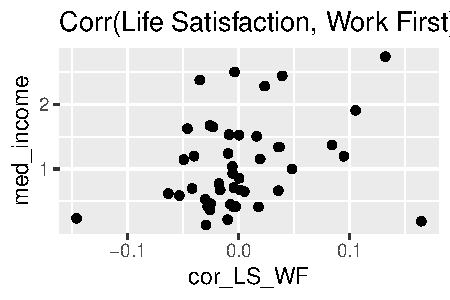
\includegraphics{TS_Modelling_files/figure-latex/unnamed-chunk-12-1.pdf}

\hypertarget{run-a-simple-regression-model}{%
\section{Run a simple regression
model}\label{run-a-simple-regression-model}}

Let's run a simple regression model with time series data.

\[ur_t = \alpha + \beta ~ rGDP_t + u_t\]

As we have quarterly GDP series we will want to reduce the frequency of
the monthly unemployment data to quarterly. the \texttt{xts} package
which we have been using to deal with the dating aspect of our data has
a handy little function to achieve this. \texttt{to.period()}.

\begin{Shaded}
\begin{Highlighting}[]
\NormalTok{ur\_female\_q }\OtherTok{\textless{}{-}} \FunctionTok{to.period}\NormalTok{(ur\_female,}\AttributeTok{period=}\StringTok{"quarters"}\NormalTok{)}
\end{Highlighting}
\end{Shaded}

As a result we get four values for each quarter (start, end, high and
low). We shall associate the last monthly unemployment rate with a
particular quarter.

\begin{Shaded}
\begin{Highlighting}[]
\NormalTok{ur\_female\_q }\OtherTok{\textless{}{-}}\NormalTok{ ur\_female\_q}\SpecialCharTok{$}\NormalTok{ur\_female.Close}
\end{Highlighting}
\end{Shaded}

We now have two quarterly series \texttt{rGDP} and
\texttt{ur\_female\_q}. We shall merge them into the same dataframe.

\begin{Shaded}
\begin{Highlighting}[]
\NormalTok{reg\_data }\OtherTok{\textless{}{-}} \FunctionTok{merge}\NormalTok{(rGDP, ur\_female\_q)}
\FunctionTok{tail}\NormalTok{(reg\_data,}\DecValTok{10}\NormalTok{)}
\end{Highlighting}
\end{Shaded}

\begin{verbatim}
##            real.GDP ur_female.Close
## 2020-09-30   503509             4.8
## 2020-12-31   509621             5.1
## 2021-03-31   504255             4.9
## 2021-06-30   537175             4.5
## 2021-09-30   546487             4.1
## 2021-12-31   554821             3.9
## 2022-03-31   557524             3.9
## 2022-06-30   557810             3.7
## 2022-09-30   557286             3.7
## 2022-12-31   558005             3.8
\end{verbatim}

By looking at the last 10 observations we can see that automatically the
dates have been matched. This is super convenient.

We can now feed these data into the \texttt{lm} function.

\begin{Shaded}
\begin{Highlighting}[]
\NormalTok{mod1 }\OtherTok{\textless{}{-}} \FunctionTok{lm}\NormalTok{(ur\_female.Close}\SpecialCharTok{\textasciitilde{}}\NormalTok{real.GDP,}\AttributeTok{data =}\NormalTok{ reg\_data)}
\FunctionTok{stargazer\_HAC}\NormalTok{(mod1)}
\end{Highlighting}
\end{Shaded}

\begin{verbatim}
## 
## =========================================================
##                              Dependent variable:         
##                     -------------------------------------
##                                ur_female.Close           
## ---------------------------------------------------------
## real.GDP                         -0.00001***             
##                                   (0.00000)              
##                                                          
## Constant                          9.829***               
##                                    (0.653)               
##                                                          
## ---------------------------------------------------------
## Observations                         123                 
## R2                                  0.271                
## Adjusted R2                         0.265                
## Residual Std. Error           1.116 (df = 121)           
## F Statistic                44.959*** (df = 1; 121)       
## =========================================================
## Note:                         *p<0.1; **p<0.05; ***p<0.01
##                     Robust standard errors in parenthesis
\end{verbatim}

This seems to suggest that higher GDP, significantly, reduces the
unemployment rate.

Let's have a look at the residuals.

\begin{Shaded}
\begin{Highlighting}[]
\FunctionTok{par}\NormalTok{(}\AttributeTok{mfrow=}\FunctionTok{c}\NormalTok{(}\DecValTok{1}\NormalTok{,}\DecValTok{2}\NormalTok{))}
\FunctionTok{plot}\NormalTok{(mod1}\SpecialCharTok{$}\NormalTok{residuals, }\AttributeTok{type =} \StringTok{"l"}\NormalTok{, }\AttributeTok{main =} \StringTok{"mod1 {-} Residuals"}\NormalTok{)}
\FunctionTok{acf}\NormalTok{(mod1}\SpecialCharTok{$}\NormalTok{residuals)}
\end{Highlighting}
\end{Shaded}

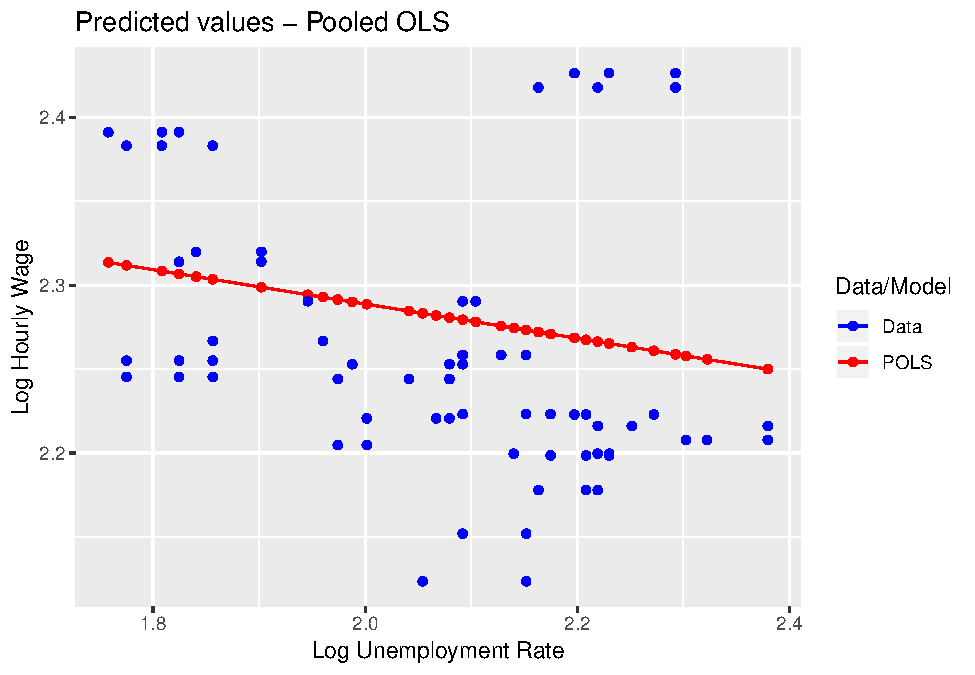
\includegraphics{TS_Modelling_files/figure-latex/unnamed-chunk-17-1.pdf}

We can see that there is a significant amount of autocorrelation in the
residuals. We can apply the Breusch-Godfrey hypothesis test
(\texttt{bgtest}). The null hypothesis is that there is no
autocorrelation.

\begin{Shaded}
\begin{Highlighting}[]
\FunctionTok{bgtest}\NormalTok{(mod1,}\AttributeTok{order=}\DecValTok{4}\NormalTok{)}
\end{Highlighting}
\end{Shaded}

\begin{verbatim}
## 
##  Breusch-Godfrey test for serial correlation of order up to 4
## 
## data:  mod1
## LM test = 116.95, df = 4, p-value < 2.2e-16
\end{verbatim}

The p-value is virtually 0 suggesting that there is stistically
significant evidence that we should reject the null hypothesis of no
autocorrelation. What is the consequence?

\hypertarget{spurious-correlations-and-regressions}{%
\section{Spurious correlations and
regressions}\label{spurious-correlations-and-regressions}}

Let's get some datasets fron EUROSTAT.

\begin{Shaded}
\begin{Highlighting}[]
\CommentTok{\# Data from EUROSTAT}
\CommentTok{\# \% of agricultural area Total fully converted and under conversion }
\CommentTok{\# to organic farming in Germany, "sdg\_02\_40"}
\CommentTok{\# Thousands of passengers travelling to and from Norway by boat, "mar\_pa\_aa"}
\CommentTok{\# Population with tertiary education (\%), "edat\_lfse\_03"}
\CommentTok{\# Hospital Discharges, Alcoholic liver disease, "NRG\_IND\_EFF"}
\CommentTok{\# The data are annual data from 2000 to 2021, 22 obs}
\NormalTok{data\_sr }\OtherTok{\textless{}{-}} \FunctionTok{read\_csv}\NormalTok{(}\StringTok{"C:/Rcode/RforQM/Time\_Series/EUROSTATtimeseries.csv"}\NormalTok{)}
\end{Highlighting}
\end{Shaded}

\begin{verbatim}
## Rows: 22 Columns: 5
## -- Column specification --------------------------------------------------------
## Delimiter: ","
## dbl (4): Year, Organic.Farming.GE, Tert.Educ.IT, Ene.Cons.PO
## num (1): Boat.Passengers.NO
## 
## i Use `spec()` to retrieve the full column specification for this data.
## i Specify the column types or set `show_col_types = FALSE` to quiet this message.
\end{verbatim}

\begin{Shaded}
\begin{Highlighting}[]
\NormalTok{dates }\OtherTok{\textless{}{-}} \FunctionTok{seq}\NormalTok{(}\FunctionTok{as.Date}\NormalTok{(}\StringTok{"2000{-}12{-}31"}\NormalTok{),}\AttributeTok{length=}\DecValTok{22}\NormalTok{,}\AttributeTok{by=}\StringTok{"years"}\NormalTok{)}
\NormalTok{data\_sr }\OtherTok{\textless{}{-}} \FunctionTok{xts}\NormalTok{(}\AttributeTok{x=}\NormalTok{data\_sr, }\AttributeTok{order.by =}\NormalTok{ dates)}
\end{Highlighting}
\end{Shaded}

I told you earlier that there are different ways to arrange several
plots in a grid. Below I present yet another (\texttt{layout} - this is
possibly the most powerful of the three as you can determine how big
each graph should be)! Don't say that this is annoying! I am merely
ramming home the message that the same thing can be done in different
ways and anyways, you will not be remembering how to do all these
things. When you want to do it you will be searching for ``R arrange
plots in grid'' or something similar. Then you will hit on any of these
methods and that is what you will adjust.

\begin{Shaded}
\begin{Highlighting}[]
\FunctionTok{layout}\NormalTok{(}\FunctionTok{matrix}\NormalTok{(}\FunctionTok{c}\NormalTok{(}\DecValTok{1}\NormalTok{,}\DecValTok{2}\NormalTok{,}\DecValTok{3}\NormalTok{,}\DecValTok{4}\NormalTok{), }\DecValTok{2}\NormalTok{, }\DecValTok{2}\NormalTok{, }\AttributeTok{byrow =} \ConstantTok{TRUE}\NormalTok{),}
   \AttributeTok{widths=}\FunctionTok{c}\NormalTok{(}\DecValTok{1}\NormalTok{,}\DecValTok{1}\NormalTok{), }\AttributeTok{heights=}\FunctionTok{c}\NormalTok{(}\DecValTok{1}\NormalTok{,}\DecValTok{1}\NormalTok{))}
\FunctionTok{plot.zoo}\NormalTok{(data\_sr}\SpecialCharTok{$}\NormalTok{Organic.Farming.GE, }\AttributeTok{ylab=}\StringTok{""}\NormalTok{, }\AttributeTok{xlab =} \StringTok{""}\NormalTok{, }\AttributeTok{main =} \StringTok{"Organic Farming}\SpecialCharTok{\textbackslash{}n}\StringTok{ GER"}\NormalTok{) }
\FunctionTok{plot.zoo}\NormalTok{(data\_sr}\SpecialCharTok{$}\NormalTok{Boat.Passengers.NO, }\AttributeTok{ylab=}\StringTok{""}\NormalTok{, }\AttributeTok{xlab =} \StringTok{""}\NormalTok{, }\AttributeTok{main =} \StringTok{"Sea Passengers}\SpecialCharTok{\textbackslash{}n}\StringTok{ NOR"}\NormalTok{)}
\FunctionTok{plot.zoo}\NormalTok{(data\_sr}\SpecialCharTok{$}\NormalTok{Tert.Educ.IT, }\AttributeTok{ylab=}\StringTok{""}\NormalTok{, }\AttributeTok{xlab =} \StringTok{""}\NormalTok{, }\AttributeTok{main =} \StringTok{"Tertiary Education}\SpecialCharTok{\textbackslash{}n}\StringTok{ ITA"}\NormalTok{)}
\FunctionTok{plot.zoo}\NormalTok{(data\_sr}\SpecialCharTok{$}\NormalTok{Ene.Cons.PO, }\AttributeTok{ylab=}\StringTok{""}\NormalTok{, }\AttributeTok{xlab =} \StringTok{""}\NormalTok{, }\AttributeTok{main =} \StringTok{"Energy Consumption}\SpecialCharTok{\textbackslash{}n}\StringTok{ POL"}\NormalTok{)}
\end{Highlighting}
\end{Shaded}

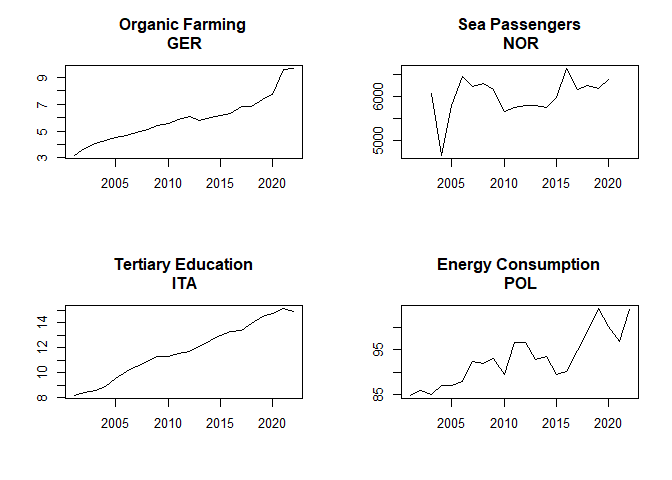
\includegraphics{TS_Modelling_files/figure-latex/unnamed-chunk-20-1.pdf}
In the above graphing commands I used \texttt{plot.zoo} and not
\texttt{ggplot} or the standard \texttt{plot}. You could have used
\texttt{ggplot} after bringing the data into long format. You could have
used the standard \texttt{plot} function. It actually does recognise
that the data are time-series data and then automatically adds all sorts
of formatting to the graphs (try by replacing \texttt{plot.zoo} with
\texttt{plot} in the above) which is rather annoying. \texttt{plot.zoo}
is a specialised plotting function for time-series data which allows
some manual finessing.

\begin{Shaded}
\begin{Highlighting}[]
\NormalTok{mod\_sr }\OtherTok{\textless{}{-}} \FunctionTok{lm}\NormalTok{(Ene.Cons.PO}\SpecialCharTok{\textasciitilde{}}\NormalTok{Organic.Farming.GE, }\AttributeTok{data =}\NormalTok{ data\_sr)}
\FunctionTok{stargazer\_HAC}\NormalTok{(mod\_sr)}
\end{Highlighting}
\end{Shaded}

\begin{verbatim}
## 
## =========================================================
##                              Dependent variable:         
##                     -------------------------------------
##                                  Ene.Cons.PO             
## ---------------------------------------------------------
## Organic.Farming.GE                2.879***               
##                                    (0.412)               
##                                                          
## Constant                          75.858***              
##                                    (2.521)               
##                                                          
## ---------------------------------------------------------
## Observations                         22                  
## R2                                  0.710                
## Adjusted R2                         0.695                
## Residual Std. Error            3.151 (df = 20)           
## F Statistic                48.874*** (df = 1; 20)        
## =========================================================
## Note:                         *p<0.1; **p<0.05; ***p<0.01
##                     Robust standard errors in parenthesis
\end{verbatim}

One way how you can unmask the spuriousness, if both series are trending
is to include a time trend

\begin{Shaded}
\begin{Highlighting}[]
\NormalTok{mod\_sr2 }\OtherTok{\textless{}{-}} \FunctionTok{lm}\NormalTok{(Ene.Cons.PO}\SpecialCharTok{\textasciitilde{}}\NormalTok{Organic.Farming.GE}\SpecialCharTok{+}\FunctionTok{index}\NormalTok{(data\_sr), }\AttributeTok{data =}\NormalTok{ data\_sr)}
\end{Highlighting}
\end{Shaded}

Now we can see that the time trend is the variable which becomes
significant and the coefficient to the organic farming variable becomes
insignificant (as it should be).

We may also want to look at running a model in the differences of
variables rather than the levels.

\begin{Shaded}
\begin{Highlighting}[]
\NormalTok{mod\_sr3 }\OtherTok{\textless{}{-}} \FunctionTok{lm}\NormalTok{(}\FunctionTok{diff}\NormalTok{(Ene.Cons.PO)}\SpecialCharTok{\textasciitilde{}}\FunctionTok{diff}\NormalTok{(Organic.Farming.GE), }\AttributeTok{data =}\NormalTok{ data\_sr)}
\FunctionTok{stargazer\_HAC}\NormalTok{(mod\_sr,mod\_sr2,mod\_sr3,}\AttributeTok{type\_out =} \StringTok{"text"}\NormalTok{, }\AttributeTok{omit.stat =} \StringTok{"f"}\NormalTok{)}
\end{Highlighting}
\end{Shaded}

\begin{verbatim}
## 
## ==========================================================================
##                                         Dependent variable:               
##                          -------------------------------------------------
##                                    Ene.Cons.PO           diff(Ene.Cons.PO)
##                                (1)             (2)              (3)       
## --------------------------------------------------------------------------
## Organic.Farming.GE          2.879***          1.145                       
##                              (0.482)         (1.872)                      
##                                                                           
## index(data_sr)                                0.001                       
##                                              (0.001)                      
##                                                                           
## diff(Organic.Farming.GE)                                      -1.242      
##                                                               (1.813)     
##                                                                           
## Constant                    75.858***       66.628***          1.291      
##                              (2.518)        (10.384)          (1.064)     
##                                                                           
## --------------------------------------------------------------------------
## Observations                   22              22               21        
## R2                            0.710           0.737            0.020      
## Adjusted R2                   0.695           0.709           -0.031      
## Residual Std. Error      3.151 (df = 20) 3.077 (df = 19)  3.547 (df = 19) 
## ==========================================================================
## Note:                                          *p<0.1; **p<0.05; ***p<0.01
##                                  Newey-West standard errors in parenthesis
\end{verbatim}

\hypertarget{run-a-simple-regression-model---but-better}{%
\section{Run a simple regression model - but
better}\label{run-a-simple-regression-model---but-better}}

Let's run a simple regression model with time series data.

\[\Delta ur_t = \alpha + \beta ~ \Delta  rGDP_t + u_t\]

As we have quarterly GDP series we will want to reduce the frequency of
the monthly unemployment data to quarterly. the \texttt{xts} package
which we have been using to deal with the dating aspect of our data has
a handy little function to achieve this. \texttt{to.period()}.

\begin{Shaded}
\begin{Highlighting}[]
\NormalTok{ur\_female\_q }\OtherTok{\textless{}{-}} \FunctionTok{to.period}\NormalTok{(ur\_female,}\AttributeTok{period=}\StringTok{"quarters"}\NormalTok{)}
\end{Highlighting}
\end{Shaded}

As a result we get four values for each quarter (start, end, high and
low). We shall associate the last monthly unemployment rate with a
particular quarter.

\begin{Shaded}
\begin{Highlighting}[]
\NormalTok{ur\_female\_q }\OtherTok{\textless{}{-}}\NormalTok{ ur\_female\_q}\SpecialCharTok{$}\NormalTok{ur\_female.Close}
\end{Highlighting}
\end{Shaded}

We now have two quarterly series \texttt{rGDP} and
\texttt{ur\_female\_q}. We shall merge them into the same dataframe.

\begin{Shaded}
\begin{Highlighting}[]
\NormalTok{reg\_data }\OtherTok{\textless{}{-}} \FunctionTok{merge}\NormalTok{(rGDP, ur\_female\_q)}
\FunctionTok{tail}\NormalTok{(reg\_data,}\DecValTok{10}\NormalTok{)}
\end{Highlighting}
\end{Shaded}

\begin{verbatim}
##            real.GDP ur_female.Close
## 2020-09-30   503509             4.8
## 2020-12-31   509621             5.1
## 2021-03-31   504255             4.9
## 2021-06-30   537175             4.5
## 2021-09-30   546487             4.1
## 2021-12-31   554821             3.9
## 2022-03-31   557524             3.9
## 2022-06-30   557810             3.7
## 2022-09-30   557286             3.7
## 2022-12-31   558005             3.8
\end{verbatim}

By looking at the last 10 observations we can see that automatically the
dates have been matched. This is super convenient.

As we will be modelling the differenced logs of the GDP and unemployment
rate it is most convenient to create these variables explicitely in the
data frame, otherwise we will have to deal with very long variable
names.

\begin{Shaded}
\begin{Highlighting}[]
\CommentTok{\# we multiply by 100 to express in percentage points, i.e. 0.5 is 0.5\% or 0.005}
\NormalTok{reg\_data}\SpecialCharTok{$}\NormalTok{d\_lgdp }\OtherTok{\textless{}{-}} \DecValTok{100}\SpecialCharTok{*}\FunctionTok{diff}\NormalTok{(}\FunctionTok{log}\NormalTok{(reg\_data}\SpecialCharTok{$}\NormalTok{real.GDP))}
\NormalTok{reg\_data}\SpecialCharTok{$}\NormalTok{d\_lur }\OtherTok{\textless{}{-}} \DecValTok{100}\SpecialCharTok{*}\FunctionTok{diff}\NormalTok{(}\FunctionTok{log}\NormalTok{(reg\_data}\SpecialCharTok{$}\NormalTok{ur\_female.Close)) }
\end{Highlighting}
\end{Shaded}

We can now feed these data into the \texttt{lm} function.

\begin{Shaded}
\begin{Highlighting}[]
\NormalTok{mod4 }\OtherTok{\textless{}{-}} \FunctionTok{lm}\NormalTok{(d\_lur}\SpecialCharTok{\textasciitilde{}}\NormalTok{d\_lgdp,}\AttributeTok{data =}\NormalTok{ reg\_data)}
\FunctionTok{stargazer\_HAC}\NormalTok{(mod4)}
\end{Highlighting}
\end{Shaded}

\begin{verbatim}
## 
## =========================================================
##                              Dependent variable:         
##                     -------------------------------------
##                                     d_lur                
## ---------------------------------------------------------
## d_lgdp                             -0.218                
##                                    (0.138)               
##                                                          
## Constant                           -0.479                
##                                    (0.375)               
##                                                          
## ---------------------------------------------------------
## Observations                         122                 
## R2                                  0.020                
## Adjusted R2                         0.012                
## Residual Std. Error           4.087 (df = 120)           
## F Statistic                  2.510 (df = 1; 120)         
## =========================================================
## Note:                         *p<0.1; **p<0.05; ***p<0.01
##                     Robust standard errors in parenthesis
\end{verbatim}

This seems to suggest that higher GDP, significantly, reduces the
unemployment rate.

Let's have a look at the residuals.

\begin{Shaded}
\begin{Highlighting}[]
\FunctionTok{par}\NormalTok{(}\AttributeTok{mfrow=}\FunctionTok{c}\NormalTok{(}\DecValTok{1}\NormalTok{,}\DecValTok{2}\NormalTok{))}
\FunctionTok{plot}\NormalTok{(mod4}\SpecialCharTok{$}\NormalTok{residuals, }\AttributeTok{type =} \StringTok{"l"}\NormalTok{, }\AttributeTok{main =} \StringTok{"mod4 {-} Residuals"}\NormalTok{)}
\FunctionTok{acf}\NormalTok{(mod4}\SpecialCharTok{$}\NormalTok{residuals)}
\end{Highlighting}
\end{Shaded}

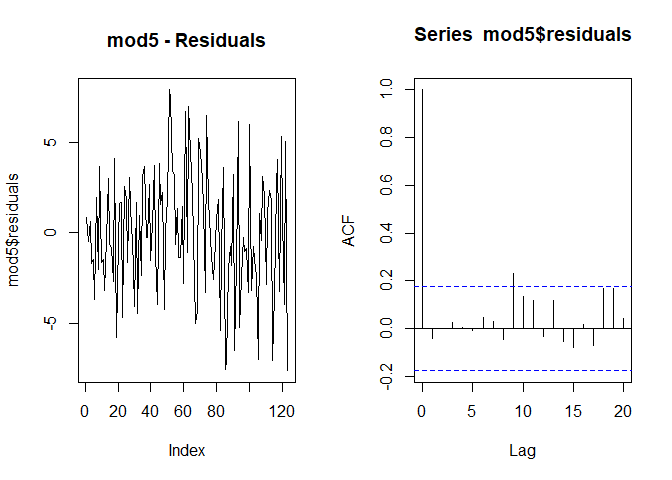
\includegraphics{TS_Modelling_files/figure-latex/unnamed-chunk-29-1.pdf}

We can see that, at lag 2, there is a small amount of autocorrelation in
the residuals. We can again apply the hypothesis test the
Breusch-Godfrey test (\texttt{bgtest}). The null hypothesis is that
there is no autocorrelation.

\begin{Shaded}
\begin{Highlighting}[]
\FunctionTok{bgtest}\NormalTok{(mod4,}\AttributeTok{order=}\DecValTok{4}\NormalTok{)}
\end{Highlighting}
\end{Shaded}

\begin{verbatim}
## 
##  Breusch-Godfrey test for serial correlation of order up to 4
## 
## data:  mod4
## LM test = 13.901, df = 4, p-value = 0.007618
\end{verbatim}

The p-value of 0.00085 suggests that there is still evidence that we
should reject the null hypothesis of no autocorrelation. What is the
consequence? Fortunately, here, despite the existence of autocorrelation
in residuals they still look stationary. We already calculated HAC
standard errors.

\hypertarget{adl-models}{%
\section{ADL Models}\label{adl-models}}

What happens if we include a lag dependent variable. Let us create the
lagged variable.

\begin{Shaded}
\begin{Highlighting}[]
\NormalTok{mod5 }\OtherTok{\textless{}{-}} \FunctionTok{lm}\NormalTok{(d\_lur}\SpecialCharTok{\textasciitilde{}}\FunctionTok{lag}\NormalTok{(d\_lur,}\DecValTok{1}\NormalTok{)}\SpecialCharTok{+}\FunctionTok{lag}\NormalTok{(d\_lur,}\DecValTok{2}\NormalTok{)}\SpecialCharTok{+}\NormalTok{d\_lgdp}\SpecialCharTok{+}\FunctionTok{lag}\NormalTok{(d\_lgdp,}\DecValTok{1}\NormalTok{)}\SpecialCharTok{+}\FunctionTok{lag}\NormalTok{(d\_lgdp,}\DecValTok{2}\NormalTok{),}\AttributeTok{data =}\NormalTok{ reg\_data)}
\FunctionTok{stargazer\_HAC}\NormalTok{(mod5)}
\end{Highlighting}
\end{Shaded}

\begin{verbatim}
## 
## =========================================================
##                              Dependent variable:         
##                     -------------------------------------
##                                     d_lur                
## ---------------------------------------------------------
## lag(d_lur, 1)                       0.070                
##                                    (0.085)               
##                                                          
## lag(d_lur, 2)                      0.197**               
##                                    (0.079)               
##                                                          
## d_lgdp                            -0.427***              
##                                    (0.122)               
##                                                          
## lag(d_lgdp, 1)                    -0.694***              
##                                    (0.131)               
##                                                          
## lag(d_lgdp, 2)                    -0.524***              
##                                    (0.130)               
##                                                          
## Constant                            0.303                
##                                    (0.334)               
##                                                          
## ---------------------------------------------------------
## Observations                         120                 
## R2                                  0.346                
## Adjusted R2                         0.317                
## Residual Std. Error           3.399 (df = 114)           
## F Statistic                12.043*** (df = 5; 114)       
## =========================================================
## Note:                         *p<0.1; **p<0.05; ***p<0.01
##                     Robust standard errors in parenthesis
\end{verbatim}

\begin{Shaded}
\begin{Highlighting}[]
\FunctionTok{par}\NormalTok{(}\AttributeTok{mfrow=}\FunctionTok{c}\NormalTok{(}\DecValTok{1}\NormalTok{,}\DecValTok{2}\NormalTok{))}
\FunctionTok{plot}\NormalTok{(mod5}\SpecialCharTok{$}\NormalTok{residuals, }\AttributeTok{type =} \StringTok{"l"}\NormalTok{,}\AttributeTok{main =} \StringTok{"mod5 {-} Residuals"}\NormalTok{)}
\FunctionTok{acf}\NormalTok{(mod5}\SpecialCharTok{$}\NormalTok{residuals)}
\end{Highlighting}
\end{Shaded}

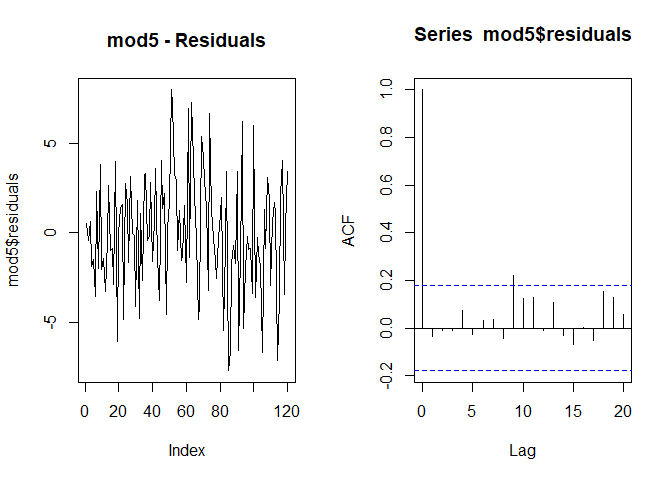
\includegraphics{TS_Modelling_files/figure-latex/unnamed-chunk-32-1.pdf}

Now the coefficient to the real GDP growth rate at time t remains
statistically insignificant, but only marginally. Most important appears
to be the unemployment rate from two quarters prior (t-2),
\texttt{lag(d\_lur,2)}.

\begin{Shaded}
\begin{Highlighting}[]
\FunctionTok{bgtest}\NormalTok{(mod5,}\AttributeTok{order=}\DecValTok{4}\NormalTok{)}
\end{Highlighting}
\end{Shaded}

\begin{verbatim}
## 
##  Breusch-Godfrey test for serial correlation of order up to 4
## 
## data:  mod5
## LM test = 2.1391, df = 4, p-value = 0.7102
\end{verbatim}

Now we remove the contemporaneous GDP growth rate.

\begin{Shaded}
\begin{Highlighting}[]
\NormalTok{mod6 }\OtherTok{\textless{}{-}} \FunctionTok{lm}\NormalTok{(d\_lur}\SpecialCharTok{\textasciitilde{}}\FunctionTok{lag}\NormalTok{(d\_lur,}\DecValTok{1}\NormalTok{)}\SpecialCharTok{+}\FunctionTok{lag}\NormalTok{(d\_lur,}\DecValTok{2}\NormalTok{)}\SpecialCharTok{+}\FunctionTok{lag}\NormalTok{(d\_lgdp,}\DecValTok{1}\NormalTok{)}\SpecialCharTok{+}\FunctionTok{lag}\NormalTok{(d\_lgdp,}\DecValTok{2}\NormalTok{),}\AttributeTok{data =}\NormalTok{ reg\_data)}
\FunctionTok{stargazer\_HAC}\NormalTok{(mod6)}
\end{Highlighting}
\end{Shaded}

\begin{verbatim}
## 
## =========================================================
##                              Dependent variable:         
##                     -------------------------------------
##                                     d_lur                
## ---------------------------------------------------------
## lag(d_lur, 1)                       0.108                
##                                    (0.088)               
##                                                          
## lag(d_lur, 2)                      0.210**               
##                                    (0.083)               
##                                                          
## lag(d_lgdp, 1)                    -0.540***              
##                                    (0.129)               
##                                                          
## lag(d_lgdp, 2)                    -0.435***              
##                                    (0.134)               
##                                                          
## Constant                            0.025                
##                                    (0.340)               
##                                                          
## ---------------------------------------------------------
## Observations                         120                 
## R2                                  0.275                
## Adjusted R2                         0.250                
## Residual Std. Error           3.562 (df = 115)           
## F Statistic                10.914*** (df = 4; 115)       
## =========================================================
## Note:                         *p<0.1; **p<0.05; ***p<0.01
##                     Robust standard errors in parenthesis
\end{verbatim}

\begin{Shaded}
\begin{Highlighting}[]
\FunctionTok{par}\NormalTok{(}\AttributeTok{mfrow=}\FunctionTok{c}\NormalTok{(}\DecValTok{1}\NormalTok{,}\DecValTok{2}\NormalTok{))}
\FunctionTok{plot}\NormalTok{(mod6}\SpecialCharTok{$}\NormalTok{residuals, }\AttributeTok{type =} \StringTok{"l"}\NormalTok{,}\AttributeTok{main =} \StringTok{"mod6 {-} Residuals"}\NormalTok{)}
\FunctionTok{acf}\NormalTok{(mod6}\SpecialCharTok{$}\NormalTok{residuals)}
\end{Highlighting}
\end{Shaded}

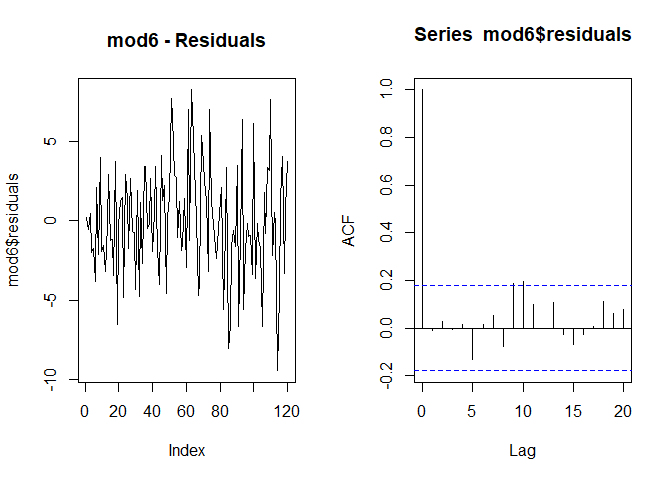
\includegraphics{TS_Modelling_files/figure-latex/unnamed-chunk-34-1.pdf}

\begin{Shaded}
\begin{Highlighting}[]
\FunctionTok{bgtest}\NormalTok{(mod6,}\AttributeTok{order=}\DecValTok{4}\NormalTok{)}
\end{Highlighting}
\end{Shaded}

\begin{verbatim}
## 
##  Breusch-Godfrey test for serial correlation of order up to 4
## 
## data:  mod6
## LM test = 1.9146, df = 4, p-value = 0.7515
\end{verbatim}

\hypertarget{autoregressive-models}{%
\section{Autoregressive Models}\label{autoregressive-models}}

Now we remove the GDP growth rate altogether from the model.

\begin{Shaded}
\begin{Highlighting}[]
\NormalTok{mod7 }\OtherTok{\textless{}{-}} \FunctionTok{lm}\NormalTok{(d\_lur}\SpecialCharTok{\textasciitilde{}}\FunctionTok{lag}\NormalTok{(d\_lur,}\DecValTok{1}\NormalTok{)}\SpecialCharTok{+}\FunctionTok{lag}\NormalTok{(d\_lur,}\DecValTok{2}\NormalTok{),}\AttributeTok{data =}\NormalTok{ reg\_data)}
\FunctionTok{stargazer\_HAC}\NormalTok{(mod7)}
\end{Highlighting}
\end{Shaded}

\begin{verbatim}
## 
## =========================================================
##                              Dependent variable:         
##                     -------------------------------------
##                                     d_lur                
## ---------------------------------------------------------
## lag(d_lur, 1)                     0.239***               
##                                    (0.089)               
##                                                          
## lag(d_lur, 2)                      0.224**               
##                                    (0.089)               
##                                                          
## Constant                           -0.340                
##                                    (0.357)               
##                                                          
## ---------------------------------------------------------
## Observations                         120                 
## R2                                  0.141                
## Adjusted R2                         0.126                
## Residual Std. Error           3.844 (df = 117)           
## F Statistic                9.617*** (df = 2; 117)        
## =========================================================
## Note:                         *p<0.1; **p<0.05; ***p<0.01
##                     Robust standard errors in parenthesis
\end{verbatim}

\begin{Shaded}
\begin{Highlighting}[]
\FunctionTok{par}\NormalTok{(}\AttributeTok{mfrow=}\FunctionTok{c}\NormalTok{(}\DecValTok{1}\NormalTok{,}\DecValTok{2}\NormalTok{))}
\FunctionTok{plot}\NormalTok{(mod7}\SpecialCharTok{$}\NormalTok{residuals, }\AttributeTok{type =} \StringTok{"l"}\NormalTok{,}\AttributeTok{main =} \StringTok{"mod7 {-} Residuals"}\NormalTok{)}
\FunctionTok{acf}\NormalTok{(mod7}\SpecialCharTok{$}\NormalTok{residuals)}
\end{Highlighting}
\end{Shaded}

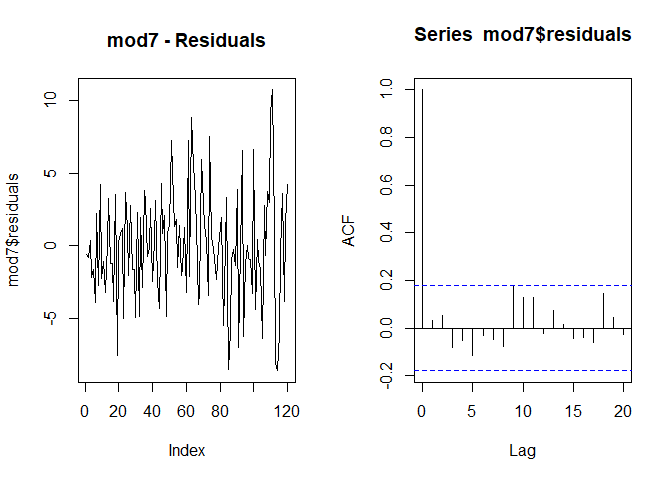
\includegraphics{TS_Modelling_files/figure-latex/unnamed-chunk-35-1.pdf}

\begin{Shaded}
\begin{Highlighting}[]
\FunctionTok{bgtest}\NormalTok{(mod7,}\AttributeTok{order=}\DecValTok{4}\NormalTok{)}
\end{Highlighting}
\end{Shaded}

\begin{verbatim}
## 
##  Breusch-Godfrey test for serial correlation of order up to 4
## 
## data:  mod7
## LM test = 2.7834, df = 4, p-value = 0.5947
\end{verbatim}

Let's look at all these models together in one table.

\begin{Shaded}
\begin{Highlighting}[]
\FunctionTok{stargazer\_HAC}\NormalTok{(mod4,mod5,mod6,mod7,}\AttributeTok{type\_out =} \StringTok{"text"}\NormalTok{, }\AttributeTok{omit.stat =} \StringTok{"f"}\NormalTok{)}
\end{Highlighting}
\end{Shaded}

\begin{verbatim}
## 
## =======================================================================================
##                                             Dependent variable:                        
##                     -------------------------------------------------------------------
##                                                    d_lur                               
##                           (1)              (2)              (3)              (4)       
## ---------------------------------------------------------------------------------------
## lag(d_lur, 1)                             0.070            0.108           0.239**     
##                                          (0.093)          (0.094)          (0.110)     
##                                                                                        
## lag(d_lur, 2)                            0.197***         0.210***         0.224**     
##                                          (0.069)          (0.074)          (0.103)     
##                                                                                        
## d_lgdp                   -0.218         -0.427***                                      
##                         (0.230)          (0.122)                                       
##                                                                                        
## lag(d_lgdp, 1)                          -0.694***        -0.540***                     
##                                          (0.073)          (0.073)                      
##                                                                                        
## lag(d_lgdp, 2)                          -0.524***        -0.435***                     
##                                          (0.068)          (0.056)                      
##                                                                                        
## Constant                 -0.479           0.303            0.025            -0.340     
##                         (0.432)          (0.317)          (0.339)          (0.413)     
##                                                                                        
## ---------------------------------------------------------------------------------------
## Observations              122              120              120              120       
## R2                       0.020            0.346            0.275            0.141      
## Adjusted R2              0.012            0.317            0.250            0.126      
## Residual Std. Error 4.087 (df = 120) 3.399 (df = 114) 3.562 (df = 115) 3.844 (df = 117)
## =======================================================================================
## Note:                                                       *p<0.1; **p<0.05; ***p<0.01
##                                               Newey-West standard errors in parenthesis
\end{verbatim}

\hypertarget{information-criteria}{%
\section{Information criteria}\label{information-criteria}}

Let's say we wanted to figure out whether it would be better to include
more lags. In addition to models \texttt{mod6} (ADL) and \texttt{mod7}
(AR), we shall estimate the equivalent models with 4 lags. In order to
then decide which model is best we look at an information criteria. This
recognises that the inclusion of additional variables (lags) will
improve the fit, but it will also reduce the precision with which the
parameters are estimated. That can be detrimental especially for
forecasting. Information criteria take this trade-off into account and
offer a way to chose the best model.

\begin{Shaded}
\begin{Highlighting}[]
\NormalTok{mod6\_4 }\OtherTok{\textless{}{-}} \FunctionTok{lm}\NormalTok{(d\_lur}\SpecialCharTok{\textasciitilde{}}\FunctionTok{lag}\NormalTok{(d\_lur,}\DecValTok{1}\NormalTok{)}\SpecialCharTok{+}\FunctionTok{lag}\NormalTok{(d\_lur,}\DecValTok{2}\NormalTok{)}\SpecialCharTok{+}\FunctionTok{lag}\NormalTok{(d\_lur,}\DecValTok{3}\NormalTok{)}\SpecialCharTok{+}\FunctionTok{lag}\NormalTok{(d\_lur,}\DecValTok{4}\NormalTok{)}\SpecialCharTok{+}
               \FunctionTok{lag}\NormalTok{(d\_lgdp,}\DecValTok{1}\NormalTok{)}\SpecialCharTok{+}\FunctionTok{lag}\NormalTok{(d\_lgdp,}\DecValTok{2}\NormalTok{)}\SpecialCharTok{+}\FunctionTok{lag}\NormalTok{(d\_lgdp,}\DecValTok{3}\NormalTok{)}\SpecialCharTok{+}\FunctionTok{lag}\NormalTok{(d\_lgdp,}\DecValTok{4}\NormalTok{),}\AttributeTok{data =}\NormalTok{ reg\_data)}
\NormalTok{mod7\_4 }\OtherTok{\textless{}{-}} \FunctionTok{lm}\NormalTok{(d\_lur}\SpecialCharTok{\textasciitilde{}}\FunctionTok{lag}\NormalTok{(d\_lur,}\DecValTok{1}\NormalTok{)}\SpecialCharTok{+}\FunctionTok{lag}\NormalTok{(d\_lur,}\DecValTok{2}\NormalTok{)}\SpecialCharTok{+}\FunctionTok{lag}\NormalTok{(d\_lur,}\DecValTok{3}\NormalTok{)}\SpecialCharTok{+}\FunctionTok{lag}\NormalTok{(d\_lur,}\DecValTok{4}\NormalTok{),}\AttributeTok{data =}\NormalTok{ reg\_data)}

\FunctionTok{stargazer\_HAC}\NormalTok{(mod6,mod7,mod6\_4,mod7\_4,}\AttributeTok{type\_out =} \StringTok{"text"}\NormalTok{, }\AttributeTok{omit.stat =} \StringTok{"f"}\NormalTok{)}
\end{Highlighting}
\end{Shaded}

\begin{verbatim}
## 
## =======================================================================================
##                                             Dependent variable:                        
##                     -------------------------------------------------------------------
##                                                    d_lur                               
##                           (1)              (2)              (3)              (4)       
## ---------------------------------------------------------------------------------------
## lag(d_lur, 1)            0.108           0.239**           0.096           0.263**     
##                         (0.094)          (0.110)          (0.114)          (0.115)     
##                                                                                        
## lag(d_lur, 2)           0.210***         0.224**          0.228**          0.273***    
##                         (0.074)          (0.103)          (0.093)          (0.093)     
##                                                                                        
## lag(d_lur, 3)                                              -0.089           -0.113     
##                                                           (0.097)          (0.114)     
##                                                                                        
## lag(d_lur, 4)                                              -0.016           -0.063     
##                                                           (0.085)          (0.083)     
##                                                                                        
## lag(d_lgdp, 1)         -0.540***                         -0.579***                     
##                         (0.073)                           (0.118)                      
##                                                                                        
## lag(d_lgdp, 2)         -0.435***                         -0.489***                     
##                         (0.056)                           (0.128)                      
##                                                                                        
## lag(d_lgdp, 3)                                             -0.141                      
##                                                           (0.153)                      
##                                                                                        
## lag(d_lgdp, 4)                                             0.087                       
##                                                           (0.148)                      
##                                                                                        
## Constant                 0.025            -0.340           0.040            -0.381     
##                         (0.339)          (0.413)          (0.341)          (0.409)     
##                                                                                        
## ---------------------------------------------------------------------------------------
## Observations              120              120              118              118       
## R2                       0.275            0.141            0.298            0.159      
## Adjusted R2              0.250            0.126            0.247            0.129      
## Residual Std. Error 3.562 (df = 115) 3.844 (df = 117) 3.599 (df = 109) 3.870 (df = 113)
## =======================================================================================
## Note:                                                       *p<0.1; **p<0.05; ***p<0.01
##                                               Newey-West standard errors in parenthesis
\end{verbatim}

\begin{Shaded}
\begin{Highlighting}[]
\FunctionTok{AIC}\NormalTok{(mod6, mod7, mod6\_4,mod7\_4)}
\end{Highlighting}
\end{Shaded}

\begin{verbatim}
## Warning in AIC.default(mod6, mod7, mod6_4, mod7_4): models are not all fitted
## to the same number of observations
\end{verbatim}

\begin{verbatim}
##        df      AIC
## mod6    6 652.3266
## mod7    4 668.6806
## mod6_4 10 647.7330
## mod7_4  6 661.1150
\end{verbatim}

We chose the model with the smallest value for the information criterion
and on this occasion this is the ADL model with 4 lags (despite lags 3
and 4 not being statistically significant).

\end{document}
